\subsection{Tipos de Sistemas}

\begin{frame}
  \frametitle{Tipos de Sistemas I}

  \vspace{-0,3cm}

  \begin{figure}
    \centering
    \small
    \begin{tikzpicture}
      \node[bloque,minimum width=15mm] (T) {T};
      \node (x) [left=of T] {};
      \node (y) [right=of T] {};
      \draw[arrow,->] (x.east) -- (T.west) node [midway,above] {$x(\cdot)$};
      \draw[arrow,->] (T.east) -- (y.west) node [midway,above] {$y(\cdot)$};
    \end{tikzpicture}
  \end{figure}
  \vspace{-0,25cm}
  \begin{itemize}
    \item <1-> Seg\'{u}n el n\'{u}mero de variables de entrada y de salida:
    \begin{itemize}
      \item \color{olivegreen}{SISO }\color{black}  (Single-Input, Single-Output): 1 variable de entrada, 1 variable de salida
      \item \alert{MIMO} (Multiple-Input, Multiple-Output): multiples variables de entrada, multiples variables de salida
      \item \alert{SIMO} (Single-Input, Multiple-Output): 1 variable de entrada, multiples variables de salida
      \item \alert{MISO} (Multiple-Input, Single-Output): multiples variables de entrada, 1 variable de salida
      \item \alert{Aut\'{o}nomo}:  sistema sin entradas de control
    \end{itemize}

    \item <2-> Según las características de la variable independiente:
    \begin{itemize}
      \item \alert{Sistemas Continuos}: admite/devuelve señales continuas
      \item \alert{Sistemas Discretos}: admite/devuelve señales discretas
      \item \alert{Conversores}: Admiten señales continuas/discretas y devuelven señales discretas/continuas
    \end{itemize}
  \end{itemize}

  \vspace{-0.4cm}

\end{frame}

%%%%%%%%%%%%%%%%%%%%%%%%%%%%%%%%%%%%%%%%%%%%

\begin{frame}
  \frametitle{Tipos de Sistemas II}

  \vspace{-0,3cm}

  \begin{figure}
    \centering
    \small
    \begin{tikzpicture}
      \node[bloque,minimum width=15mm] (T) {T};
      \node (x) [left=of T] {};
      \node (y) [right=of T] {};
      \draw[arrow,->] (x.east) -- (T.west) node [midway,above] {$x(\cdot)$};
      \draw[arrow,->] (T.east) -- (y.west) node [midway,above] {$y(\cdot)$};
    \end{tikzpicture}
  \end{figure}

  \vspace{-0.25cm}

  \begin{itemize}
    \item <1-> Seg\'{u}n la existencia o no de procesos aleatorios:
    \begin{itemize}
      \item \alert{Sistemas Deterministas}: no hay procesos aleatorios involucrados, por lo que la respuesta del sistema ante la mismas entradas es siempre la misma.
      \item \alert{Sistemas Estoc\'{a}sticos}: hay procesos aleatorios involucrados, por lo que la respuesta del sistema ante la mismas entradas depende del experimento.
    \end{itemize}

    \item <2-> Causales/no causales:
    \begin{itemize}
      \item \color{olivegreen}{Sistemas Causales}\color{black}: La salida del sistema en un instante únicamente depende de las entradas hasta dicho instante de tiempo. 

  \vspace{0.2cm}

     \hspace{0.4cm} $y(t)=\bm{T} [ \:x(\tau)|\tau<=t\: ] \: \:$       ó          $\: \:y[n]=\bm{T}[\: x[k]|k<=n\:]$ 
     
     \vspace{0.2cm}
     
      \item \alert{Sistemas No Causales}: La salida del sistema en un instante depende de la entrada en instantes posteriores. No es físicamente realizable. 
    \end{itemize}

  \end{itemize}

\vspace{-0.4cm}

\end{frame}

% %%%%%%%%%%%%%%%%%%%%%%%

\begin{frame}
\frametitle{Tipos de Sistemas III}

\vspace{-0,1cm}

\begin{figure}
  \centering
  \small
  \begin{tikzpicture}
    \node[bloque,minimum width=15mm] (T) {T};
    \node (x) [left=of T] {};
    \node (y) [right=of T] {};
    \draw[arrow,->] (x.east) -- (T.west) node [midway,above] {$x(\cdot)$};
    \draw[arrow,->] (T.east) -- (y.west) node [midway,above] {$y(\cdot)$};
  \end{tikzpicture}
  \end{figure}

  \vspace{-0.25cm}
  \begin{itemize}
    \item <1-> Respecto a la memoria del sistema:
    \begin{itemize}
      \item \alert{Sistemas Estáticos}: La salida del sistema en un instante depende únicamente de la entrada en dicho instante. 
  
      \vspace{0.1cm}
      \hspace{1cm}    $y(t)=\bm{T}[\:x(t)\:] \: \:$       ó          $\: \:y(n)=\bm{T}[\:x[n]\:]$ 
  
      \vspace{0.1cm}    
      \item \color{olivegreen}{Sistemas Dinámicos}\color{black}: La salida del sistema en un instante depende de la historia pasada del sistema. Los sistemas dinámicos continuos se pueden modelar con una ecuación diferencial. Los discretos con una ecuación en diferencias.

      \vspace{0.1cm}

      $y(t)=\bm{T}[\:x(\tau) | \tau \subseteq \mathbb{R} \le t\:] \: \:$       ó          $\: \:y(n)=\bm{T}[\:x[k] | k \subseteq \mathbb{Z} \le n\:]$
      \vspace{0.1cm}
 
    \end{itemize}

    \item <2-> Estable/inestable:
    \begin{itemize}
      \item \color{olivegreen}{Sistemas Estables}\color{black}: cuando responde con una salida acotada en amplitud ante cualquier entrada acotada (BIBO-estable: bounded-input, bounded-output). 

      \vspace{0.1cm}

      \hspace{1.8cm} $|x(\cdot)|< B_1  \rightarrow  |y(\cdot)|< B_2$  
     
      \vspace{0.1cm}
      \item \alert{Sistemas Inestables}\color{black}: cuando no cumplen la propiedad anterior. 


    \end{itemize}

%\item <1-> Invertibles/no invertibles:
%\begin{itemize}
%\item \alert{Sistemas Invertibles}\color{black}: en los que  existe una función $\bm{T}^{-1}[\cdot]$ que permite recuperar la entrada a partir de la salida. 

%  \vspace{0.1cm}

%     \hspace{1.8cm} $x(\cdot)=\bm{T}^{-1} [\: \bm{T}[\:x(\cdot)\: ]  \: ]$  
     
% \vspace{0.1cm}
     

     
%\item \alert{Sistemas No Invertibles}: en los que no existe la función $\bm{T}^{-1}[\cdot]$.
%\end{itemize}
  \end{itemize}
\end{frame}

% %%%%%%%%%%%%%%%%%




\begin{frame}
  \frametitle{Tipos de Sistemas IV}

  \vspace{-0.4cm}

  \begin{columns}[c]
    \hspace{-1.8cm}\begin{column}{12cm}
      \small 
      \begin{itemize}
        \item <1-> Sistemas lineales/no lineales:
        \begin{itemize}
          \item \color{olivegreen}{Sistemas Lineales}\color{black}: Los que cumplen el principio de superposición, i.e. la respuesta del sistema producido por varias fuentes excitadoras a la vez es la suma de las respuestas producidas por las fuentes individualmente.
          \vspace{0.1cm}
          $\bm{T}[\:\alpha x_1(\cdot)+\beta x_2(\cdot)\:]=\alpha \bm{T}[\:x_1(\cdot)\:] + \beta \bm{T}[\: x_2(\cdot) \:] =\alpha y_1(\cdot)+ \beta y_2(\cdot)$
          \vspace{0.1cm}
          \item \alert{Sistemas No Lineales}: Los que no cumplen el principio de superposición. Los sistemas reales son sistemas no lineales, aunque pueden ser tratados como sistemas lineales en torno a un determinado punto de operaci\'{o}n.
        \end{itemize}
      \end{itemize}
    \end{column}
    \hspace{-7cm}\begin{column}{4cm}
      \vspace{-3.75cm}
      \small
      \begin{tikzpicture}
        \node[bloque,minimum width=15mm] (T) {T};
        \node (x) [left=of T] {$x(\cdot)$};
        \node (y) [right=of T] {$y(\cdot)$};
        \draw[arrow,->] (x.east) -- (T.west);
        \draw[arrow,->] (T.east) -- (y.west);
      \end{tikzpicture}
    \end{column}
  \end{columns}
  \vspace{0.2cm}
  \begin{columns}[c]
    \begin{column}{4cm}
      \includegraphics[width=3.8cm]{./Figuras/FigLT1.eps} 
    \end{column}
    \begin{column}{4cm}
      \includegraphics[width=3.8cm]{./Figuras/FigLT2.eps} 
    \end{column}
    \begin{column}{4cm}
      \includegraphics[width=3.8cm]{./Figuras/FigLT3.eps} 
    \end{column}
  \end{columns}
\end{frame}

%%%%%%%%%%%%%%%%%%%%%%%%%%%%%%%%

\begin{frame}
  \frametitle{Tipos de Sistemas V}
  \small
  \vspace{-0.4cm}

  \begin{columns}[c]
    \hspace{-0.2cm}\begin{column}{12cm}
      \begin{itemize}
        \item <1-> Sistemas temporalmente invariantes/no invariantes:
        \vspace{-0.2cm}
        \begin{itemize}
          \item \color{olivegreen}{Sistemas Temporalmente  Invariantes}\color{black}: Aquellos en los que su relación entrada-salida es invariante en el tiempo (a una entrada desplazada temporalmente le corresponde la misma salida desplazada el mismo valor).
          \vspace{0.1cm}
          $\bm{T}[\: x(t)\:]=y(t) \rightarrow \bm{T}[\: x(t-t_0)\:]=y(t-t_0)$
          \vspace{0.1cm}
          $\bm{T}[\: x[n]\:]=y(n) \rightarrow \bm{T}[\: x(n-N_0)\:]=y(n-N_0)$
          \vspace{0.1cm}
          \item \alert{Sistemas Temporalmente No  Invariantes}: Los que no cumplen la propiedad anterior.
      \end{itemize}

      \begin{columns}[c]
        \begin{column}{4cm}
          \includegraphics[width=4cm]{./Figuras/FigLT1B.eps} 
        \end{column}
        \begin{column}{4cm}
          \includegraphics[width=4cm]{./Figuras/FigLT2B.eps} 
        \end{column}
      \end{columns}

      \vspace{-0.2cm}
      \item \color{olivegreen}{Sistemas Lineales Temporalmente Invariantes}: Sistemas LTI
      \end{itemize}
    \end{column}
    \hspace{-3.0cm}\begin{column}{4cm}
      \vspace{7.25cm}
      \small
      \begin{tikzpicture}[scale=0.8,every node/.style={scale=0.8}]
        \node[bloque,minimum width=15mm] (T) {T};
        \node (x) [left=of T] {};
        \node (y) [right=of T] {};
        \draw[arrow,->] (x.east) -- (T.west) node [midway,above] {$x(\cdot)$};
        \draw[arrow,->] (T.east) -- (y.west) node [midway,above] {$y(\cdot)$};
      \end{tikzpicture}
    \end{column}
  \end{columns}

\end{frame}